%%%%%%%%%%%%%%%%%%%%%%%%%%%%%%%%%%%%%%%%%%%%%%%%%%%%%%%%%%
% benchmarks.tex
%%%%%%%%%%%%%%%%%%%%%%%%%%%%%%%%%%%%%%%%%%%%%%%%%%%%%%%%%%

Our system is mainly concerned with optimizing away the overhead that dynamically building and maintaining an X3D scene produces. To show that we have achieved our objective, we have tested the same scene on multiple browsers and profiled the resulting framerates. The browsers we have used are BS Contact and Octaga.

We have tested for scenes with a relatively low number of shapes (300 and 680). We are not really interested in testing the rendering performance, since such a test would mainly compare the efficiency of the underlying rendering APIs and would not be relevant in this context. Both scenes are compared against two other scenes with the same shapes but with 3 \texttt{color interpolators}, 2 \texttt{timers} and 6 \texttt{routes} for each shape. The resulting routing and logic are quite heavy and constitutes a good test the underlying execution model for routes and logical nodes.

The tables below show a comparison in performance for each browser with various hardware configurations:

\begin{table}[htb]
\centering
\begin{tabular}{|l|c|c|c|}
\hline
Browser & FPS & FPS (with routes) & Diff \% 	 \\
\hline
XNA (300 shapes) & 580 & 510 & -12 \\
XNA (680 shapes) & 265 & 224 & -15 \\
Octaga (300 shapes) &  670 & 340 & -49 \\
Octaga (680 shapes) &  372 & 150 & -60 \\
BS C. (300 shapes) & 370 & 300 & -19 \\
BS C. (680 shapes) & 185 & 145 & -22 \\
\hline
\end{tabular}
\caption{Intel E6300, 3 GB RAM, nVidia GT 240}
\end{table}

\begin{table}[htb]
\centering
\begin{tabular}{|l|c|c|c|}
\hline
Browser & FPS & FPS (with routes) & Diff \% 	 \\
\hline
XNA (300 shapes) & 670 & 590 & -12 \\
XNA (680 shapes) & 310 & 265 & -15 \\
BS C. (300 shapes) & 530 & 368 & -31 \\
BS C. (680 shapes) & 285 & 146 & -49 \\
\hline
\end{tabular}
\caption{Intel Core i5, 8 GB RAM, nVidia 310M}
\end{table}

\begin{table}[htb]
\centering
\begin{tabular}{|l|c|c|c|}
\hline
Browser & FPS & FPS (with routes) & Diff \% 	 \\
\hline
XNA (300 shapes) & 640 & 600 & -6 \\
XNA (680 shapes) & 310 & 280 & -10 \\
Octaga (300 shapes) &  720 & 403 & -44 \\
Octaga (680 shapes) &  345 & 181 & -48 \\
BS C. (300 shapes) & 500 & 360 & -28 \\
BS C. (680 shapes) & 215 & 135 & -37 \\
\hline
\end{tabular}
\caption{Intel E8500, 2 GB RAM, ATI HD 4800}
\end{table}

\begin{figure}
\begin{center}
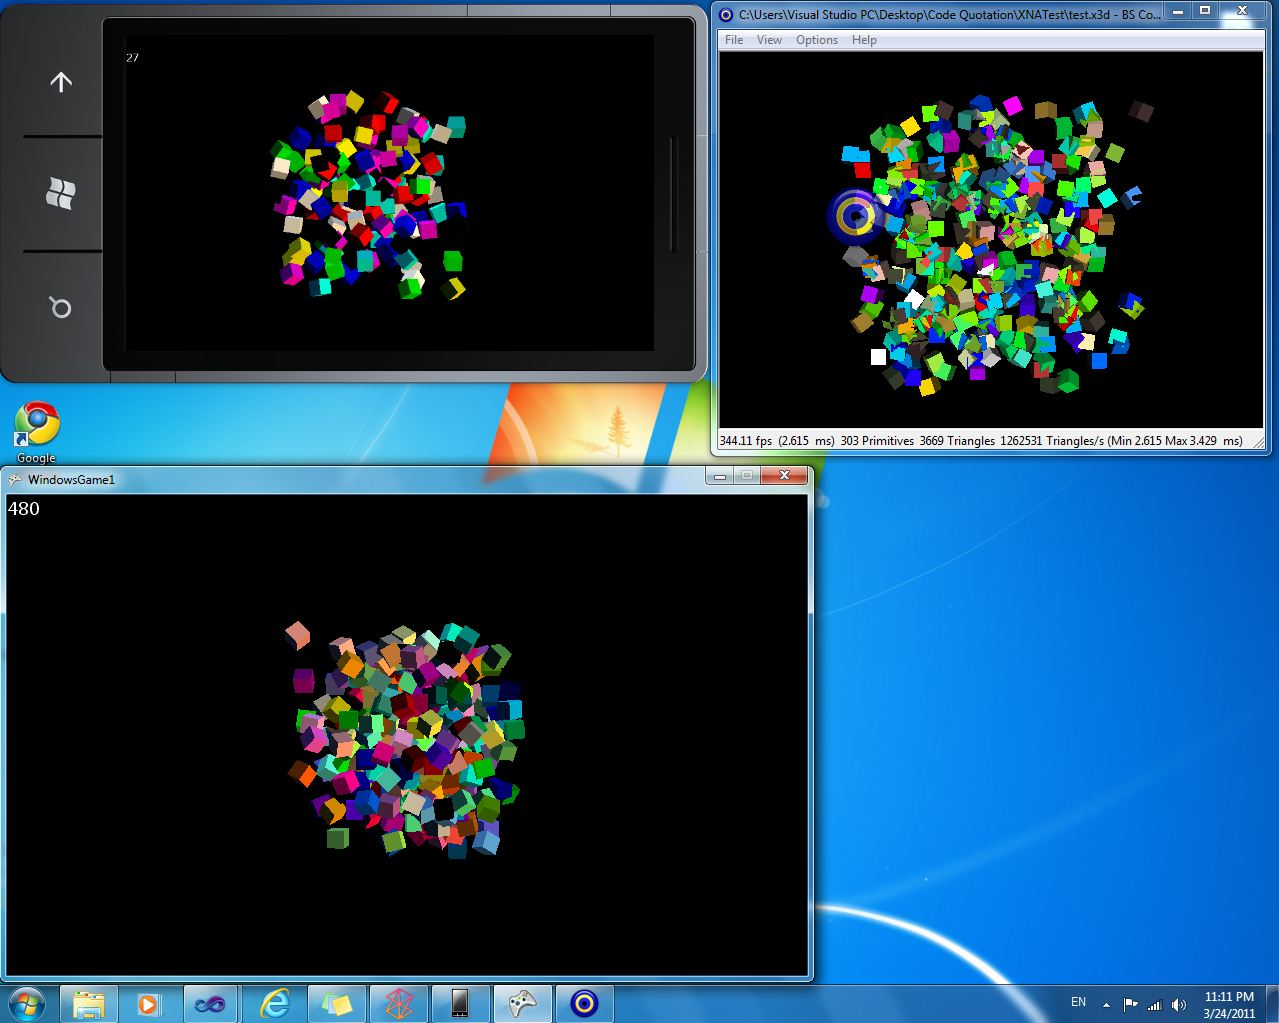
\includegraphics[scale=0.2]{browsers.jpg}
\end{center}
\caption{WP7 Emulator, BS Contact and XNA Windows Application}
\end{figure}

It is clear that thanks to our approach the scene logic weighs far less than it does in the other browsers.

Moreover, as we can see in Fig �3, the code that is generated by our system can be run, \textit{without modification} also in Windows Phone 7 devices; in the figure we can see the emulator in action. The results of running two compiled scenes with 150 and 300 shapes respectively plus the usual routes for each shape are summarized in the table below:

\begin{table}[htb]
\centering
\begin{tabular}{|l|c|}
\hline
Scene & FPS 	 \\
\hline
150 shapes with routes & 30 \\
300 shapes with routes & 24 \\
\hline
\end{tabular}
\caption{WP7 (LG Optimus 7)}
\end{table}



At this point we have completed supporting the static aspects of an X3D scene, those that are involved in nodes that are not added or removed dynamically. This approach clearly yields an increase in performance for scenes with a complex logic in terms of timers, routes, interpolators, etc. We now move to the second part of our work, which focuses on integrating our compiled scenes with scripts that can implement nodes that are added or removed dynamically and any other aspect of the scene that would be hard to express in plain X3D.
